% flashcards-title: Projection onto a direction
% flashcards-desc: A five-centimetre vector makes sixty degrees with the b-hat direction and drops a perpendicular projection guide.
\documentclass[border=7pt]{standalone}
\def\pgfsysdriver{pgfsys-dvisvgm.def}
\usepackage{tikz}
\usetikzlibrary{arrows.meta,positioning,shapes.geometric}
\definecolor{mechInk}{HTML}{172033}
\definecolor{mechBlue}{HTML}{155EEF}
\definecolor{mechOrange}{HTML}{B54708}
\definecolor{mechPale}{HTML}{E8F0FF}
\definecolor{mechGray}{HTML}{667085}
\definecolor{mechLight}{HTML}{D0D5DD}
\tikzset{
  every picture/.style={font=\sffamily\large, text=mechInk},
  mech box/.style={draw=mechInk, line width=1.2pt, rounded corners=4pt,
    fill=white, align=center, minimum height=14mm, inner xsep=5mm},
  mech primary/.style={draw=mechBlue, line width=2.2pt},
  mech secondary/.style={draw=mechOrange, line width=2.2pt, dashed},
  mech guide/.style={draw=mechGray, line width=0.9pt, dashed},
  mech arrow/.style={-{Stealth[length=3.2mm,width=2.4mm]},
    draw=mechInk, line width=1.4pt, line cap=butt},
  mech axis/.style={draw=mechInk, line width=1.2pt},
  mech tick/.style={draw=mechInk, line width=1pt}
}

\begin{document}
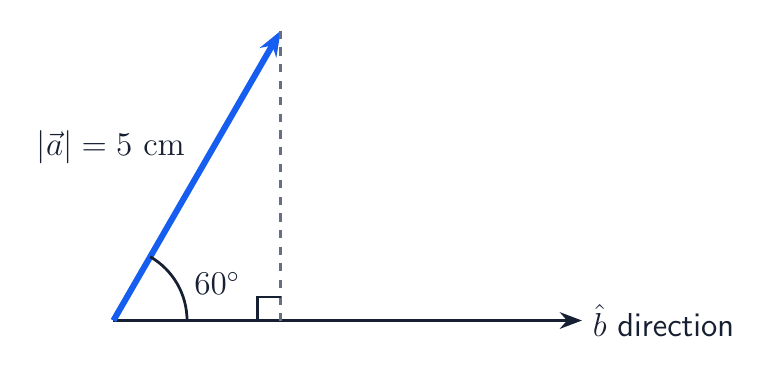
\begin{tikzpicture}[x=0.85cm,y=0.85cm]
  \draw[mech axis,-{Stealth[length=2.8mm,width=2.1mm]}] (0,0) -- (7,0) node[right] {$\hat b$ direction};
  \draw[mech primary,-{Stealth[length=3.2mm,width=2.4mm]},line cap=butt] (0,0) -- (2.5,4.33) node[midway,above left] {$|\vec a|=5\ \mathrm{cm}$};
  \draw[mech guide] (2.5,4.33) -- (2.5,0);
  \draw[mechInk,line width=1pt] (1.1,0) arc[start angle=0,end angle=60,radius=1.1];
  \node at (1.55,0.55) {$60^\circ$};
  \draw[mechInk,line width=0.9pt] (2.5,0.35) -- (2.15,0.35) -- (2.15,0);
\end{tikzpicture}
\end{document}
